\section{From Rules to Chaos}
\label{sec:chaos}

We have seen simple processes like the Golden Mean, which require only a few bits of memory. But what happens when we look at complex physical systems?

One of the most surprising discoveries of the 20th century was \textbf{Chaos}: simple deterministic rules can produce behavior that looks completely random. Computational Mechanics gives us a toolkit to "measure" this chaos. It allows us to ask: \textit{Is this randomness "simple" (like a coin flip) or "complex" (requiring memory)?}

\subsection{The Logistic Map}
Consider a simple model of population growth, the Logistic Map:
\[ x_{n+1} = r x_n (1 - x_n) \]
where $x_n$ is the population at year $n$, and $r$ is the growth rate.

As we increase $r$, the behavior undergoes a dramatic transformation:
\begin{itemize}
    \item \textbf{Order ($r < 3$)}: The population settles to a single stable value.
    \item \textbf{Periodicity ($r \approx 3.5$)}: The population bounces between 2, 4, 8... values.
    \item \textbf{Chaos ($r \approx 4.0$)}: The population jumps wildly and unpredictably.
\end{itemize}

\subsection{The Structure of Chaos}
We can convert this numerical data into symbols: '1' if the population is high ($x > 0.5$), '0' if low. Then, we use \texttt{emic} to infer the $\epsilon$-machine at each value of $r$.

\begin{emiclisting}[label=lst:chaos]{Scanning for Chaos}
\begin{lstlisting}[language=Python, basicstyle=\tiny\ttfamily, numbers=none]
# Scan the parameter r
for r in np.linspace(3.5, 4.0, 100):
   data = logistic_map(r, size=10000)
   machine = cssr.infer(data)
   # How much memory does the process need?
   complexity = machine.statistical_complexity()
\end{lstlisting}
\end{emiclisting}

The results, shown in Figure \ref{fig:logistic}, reveal the hidden architecture of chaos.

\begin{emicfigure}[float*=t, label=fig:logistic]{The Architecture of Chaos}
    \centering
    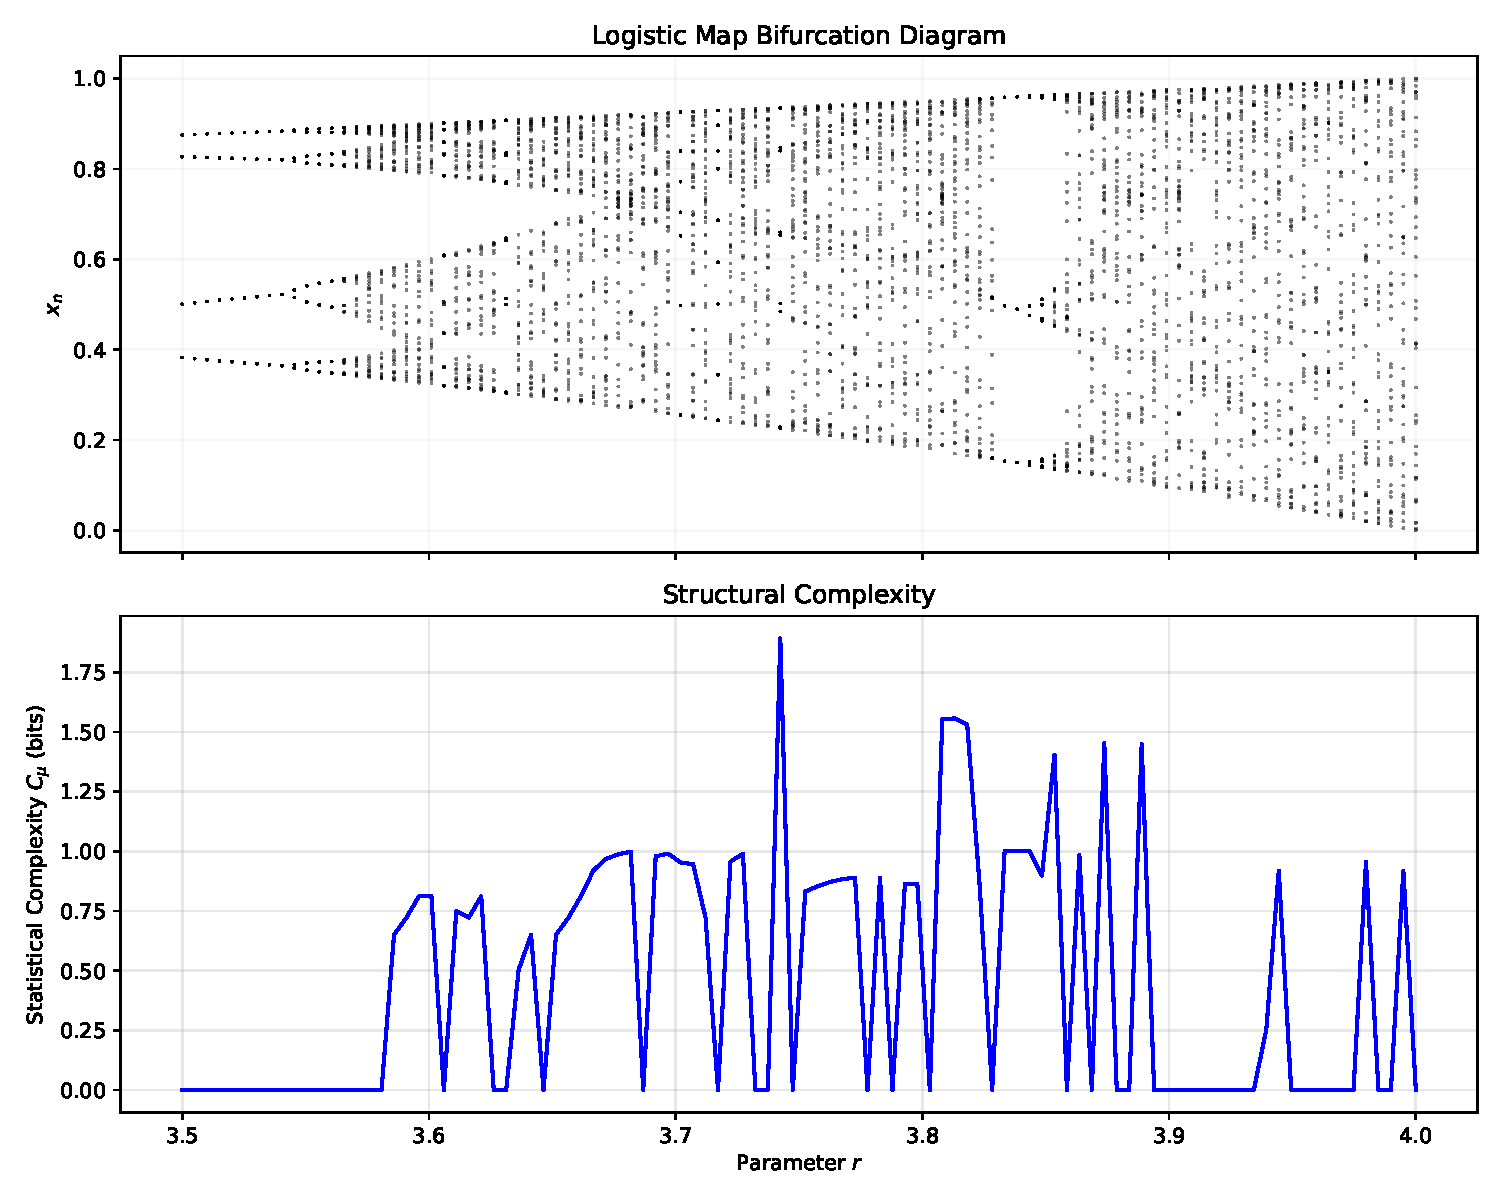
\includegraphics[width=\textwidth]{figures/logistic_complexity.pdf}

    Top: The bifurcation diagram (values of $x$). Bottom: Structural complexity ($C_\mu$).
\end{emicfigure}

\begin{intuition}
    \textbf{The Edge of Chaos}\\
    Look at the blue curve (Statistical Complexity).
    \begin{itemize}
        \item In the \textbf{Ordered} regime, complexity is low. It's easy to predict a fixed point.
        \item In the \textbf{Chaotic} regime (far right), complexity is \textit{also} low! If a system is completely random, you don't need memory to predict it---you just guess.
        \item The peaks occur at the \textbf{transition}, the "Edge of Chaos".
    \end{itemize}
    This tells us something profound: \textbf{Structure lives in the balance between order and randomness.}
\end{intuition}
